%!TEX root = mainfile.tex
\section{Spectroscopy} % (fold)
\label{sec:spectroscopy}
	The spectrum of typical high redshift galaxy can be seen in Figure~\ref{fig:high_redshift_galaxy_spectrum}.
	\begin{figure}[!htbp]
		\centering
			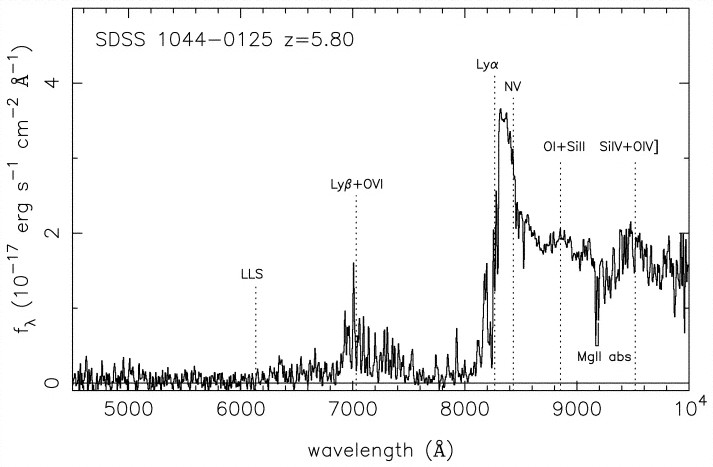
\includegraphics[width=0.7\textwidth]{../Images/high_redshift_galaxy_spec.jpg}
		\caption{\label{fig:high_redshift_galaxy_spectrum}}
	\end{figure}

	The distinct drop in emission is due to the presence of neutral hydrogen around the galaxies, known as the Gunn Peterson trough. Therefore the galaxies where formed before the start of re-ionisation. This is discussed in detail in Section~\ref{sec:the_gunn_peterson_effect}. However this particular feature in the spectra is of great importance here. The wavelength at which this drop occurs corresponds to the amount of energy required for an electron to transition between the first two energy levels in neutral hydrogen. This is known as the Lyman-$\alpha$ transition line and has a rest frame wavelength here on earth of \SI{1216}{\angstrom}\cite{}[1][2]. However, the actual wavelength that this drop occurs in the spectrum of the galaxy being studied will be much longer. In Figure~\ref{fig:high_redshift_galaxy_spectrum}, it is closer to \SI{8000}{\angstrom}.This is due to the fact that the light is red shifted effectively stretching the wavelength. Indeed, the observed wavelength of the Lyman-$\alpha$ transition line will be in the infrared range. If this wavelength can be measured precisely then the redshift of the galaxy can be calculated\cite{}[2]. This is done using the relation,
	\begin{align}
		1+z &= \frac{\lambda_{\text{observed}}}{\lambda_{\text{emitted}}} \label{eq:spectroscopy}
	\end{align}
	Hence, spectroscopy can be used to confirm the high-red shift galaxy candidates that are identified via photometry. In essence it is high resolution photometry.

	An astronomical spectrograph splits or disperses light from a source into its constituent wavelengths. Therefore it has to have some means of dispersing the light. The simplest way this can be achieved is via a prism. This exploits the fact that different wavelengths are diffracted via different amounts. However, they are rarely used by themselves in astronomical spectroscopy due to their inefficiency. Only about 10\% of the light incident upon them actually gets dispersed. Moreover, the dispersion is nonlinear causing some light to be dispersed more than others. Therefore, the universal dispersing medium used in astronomical spectroscopy is the diffraction grating. A diffraction grating consists of a large number of equidistant parallel lines ruled onto a transparent glass plate. The incident light cannot travel through the grating, but is instead channelled along the parallel lines. As the light reaches the end of the lines it is diffracted producing a series of wavelets in accordance with Huygens’s Principle. These either constructively or destructively interfere producing a series of maxima or minima. Again, different wavelengths of light will be diffracted through different angles. Therefore each maximum (order) can be thought of as the image of the galaxy split into its constituent wavelengths. As a general rule, the first maximum is projected onto the CCD equipment of the telescope and used to calculate the redshift. This is due to the fact it has the highest intensity. Figures~\ref{fig:grating_to_split_light} and~\ref{fig:grating_close_up} below show a schematic of a grating being used to split light
	\begin{figure}[!htbp]
		\begin{minipage}[c]{0.5\linewidth}
			\centering
			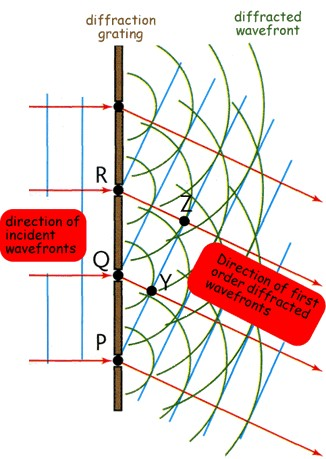
\includegraphics[width=0.7\textwidth]{../Images/grating_to_split_light.jpg}
			\caption{\label{fig:grating_to_split_light}}
		\end{minipage}
		\begin{minipage}[c]{0.5\linewidth}
			\centering
			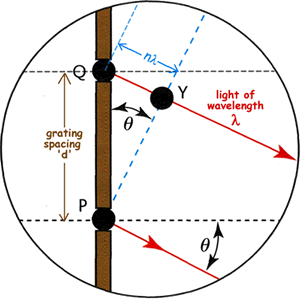
\includegraphics[width=0.7\textwidth]{../Images/grating_close_up.png}
			\caption{\label{fig:grating_close_up}}
		\end{minipage}
	\end{figure}

	Angles at which the orders occur can be found using the grating equation,
	\begin{align}
		n\lambda &= d(\sin\theta + \sin\phi)
	\end{align}
	Where $\phi$ is the angle of incidence between the light and the grating, $\theta$ is the angle of dispersion and $d$ is the grating spacing. The value of $n\lambda$ is an integer number of wavelengths of the incident light.

	Before light reaches either a prism or diffraction grating it is often sent through a fixed slit. This is a mask with a narrow rectangular aperture that is placed in the focal plane of the telescope. The slit has two main functions. First and foremost it isolates a portion of the sky of interest so that only light that falls on the slit may enter the spectrograph. This is important as it means the spectra from different parts of a galaxy cannot enter the spectrograph, overlap and thus contaminate each other. Second, the slit provides a stable spectral resolution. Without the slit the spectral resolution would be defined by the width of the galaxy or star. However, this varies with time so the spectral line width would vary with time. This would make detailed analysis of the spectrum almost impossible. If on the other hand a slit is used, the spectrum becomes an infinite number of images of the slit, and not the galaxy or star etc. As the slit width is constant, the spectral resolution remains stable.

	In between the slit and dispersion medium usually sits a collimator. The light from the slit diverges and if left would hit the grating or prism at differing angles of incidence making the resulting spectrum useless. Therefore a collimator is used to turn the diverging light back to parallel. Figure~\ref{fig:nirspec_jwst} below shows the set-up for NIRspec on the JWST.
	\begin{figure}[!htbp]
		\centering
			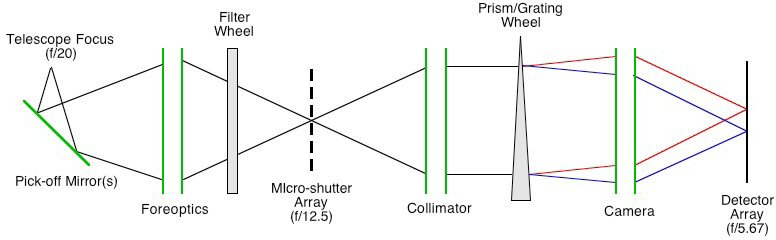
\includegraphics[width=0.8\textwidth]{../Images/nirspec_jwst.jpeg}
		\caption{\label{fig:nirspec_jwst}}
	\end{figure}

	\subsection{Candidate Telescopes} % (fold)
	\label{sub:candidate_telescopes}
		\subsubsection{James Webb Space Telescope} % (fold)
		\label{ssub:james_webb_space_telescope}
			The primary telescopes considered for use in this research are the JWST and the E-ELT. The JWST’s NIRSpec is a device which will enable the conformation of high red shift galaxies. It uses a combination of slits, prims and gratings to achieve high resolution spectroscopy. Perhaps its most innovative feature is a microshutter array. The microshutters are tiny cells that measure $100 \times 200$\,\si{\micro\metre}. They are arranged over a waffle like grid containing \num{62000} individual cells. NIRSpec will contain four identical grids in total. The cells all have lids which can be opened and closed individually. This is achieved by sweeping a magnet across the surface of the array which opens all of the lids and the electronically closing individual lids. Each cell measures $203 \times 463$\,milliarcseconds. The total field of view for all four arrays combined is $3 \times 3$\,arcminutes. Shutters in each array can be opened or closed to form multiple apertures meaning that spectrums for one hundred different targets can be found simultaneously. The size and shape of the apertures can be selected to obtain the clearest spectrum possible for each individual target. Figures~\ref{fig:nirspec_construction} and~\ref{fig:nirspec_mirrors} show NIRSpec under construction\cite{}[7] \cite{}[8].
			\begin{figure}[!htbp]
				\begin{minipage}[c]{0.5\linewidth}
					\centering
					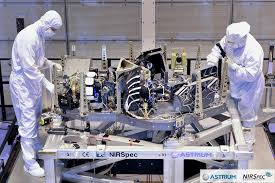
\includegraphics[width=0.9\textwidth]{../Images/nirspec_construction.jpeg}
					\caption{\label{fig:nirspec_construction}}
				\end{minipage}
				\begin{minipage}[c]{0.5\linewidth}
					\centering
					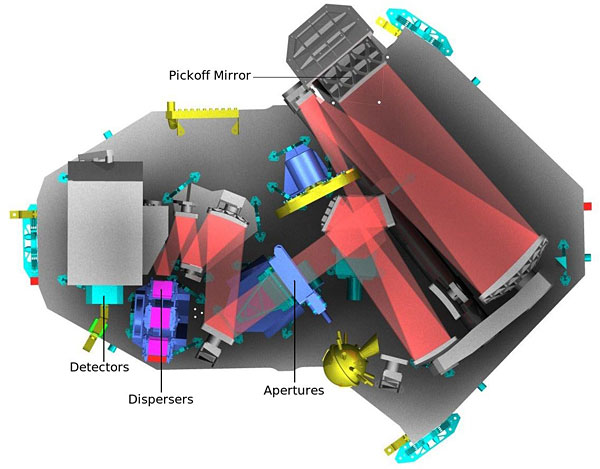
\includegraphics[width=0.9\textwidth]{../Images/nirspec_mirrors.jpeg}
					\caption{\label{fig:nirspec_mirrors}}
				\end{minipage}
			\end{figure}

			As well as the microshutter array the JWST also contains an integral field unit. Integral field spectroscopy has become an important sub discipline of astronomy where there is a need to study the spectra of extended bodies. This has particular significance as high red shift galaxies are considered to be extended bodies.

			Integral field spectroscopy is the successor to long slit spectroscopy where the spectrum is dispersed perpendicular to the slit direction. By stepping the position of the slit the spectrum of points over the extended body can be obtained. An integral field unit speeds up this process by slicing the image and then rearranging it so that different parts can illuminate the slit. This negates the need to take multiple exposures\cite{}[9]\cite{}[10].

			NIRSpec will be able to disperse light comprised of wavelengths between 0.6 and 5 microns, i.e. the infrared range over which the Gunn Peterson trough should occur. It will do this using one prism and five diffraction gratings. The wavelength ranges over which each will work and their associated wavelengths are shown below\cite{}[11].
			\begin{table}[!htbp]
				\begin{center}
					\begin{tabular}{c|c|c|c}
						Grating & Filter & Resolution & Wavelength (\si{\micro\metre}) \\
						\hline \hline
						Prism & Clear & 100 & 0.5--5 \\
						G140M & F100LP & 1000 & 1.0--1.8 \\
						G235M & F170LP & 1000 & 1.7--3.0 \\
						G395M & F290LP & 1000 & 2.9--5.0 \\
						G140M & F100LP & 2700 & 1.0--1.8 \\
						G235M & F170LP & 2700 & 1.7--3.0 \\
						G395M & F290LP & 2700 & 2.9--5.0
					\end{tabular}
				\end{center}
				\caption{Number of galaxies for set total observing time given different magnitudes/ survey areas for JWST.\label{tab:galaxies_for_set_total_observing_time_JWST}}
			\end{table}
		% subsubsection james_webb_space_telescope (end)

		\subsection{European Extremely Large Telescope} % (fold)
		\label{sub:european_extremely_large_telescope}
			The European-Extremely Large Telescope (E-ELT) will be equipped with three spectroscopic devices:
			\begin{enumerate}
				\item EAGLE - A multichannel integral field near infrared spectrograph with multi object adaptive optics;
				\item HARMONI - A wide band field spectrograph;
				\item SIMPLE – Echelle high resolution spectrograph.
			\end{enumerate}
			EAGLE will enable spectrums of multiple galaxies to be obtained simultaneously and thus would be of great benefit for this project. However, as it is only in early development stage information required to perform estimates for exposure times is not available. It is most likely to use a system of fibre optics to stack spectrums of galaxies onto the CCD. The fibre optics will sit between the diffraction grating and the CCD. As mentioned above it will use a system of multi object adaptive objects. This will use separate pieces of a deformable mirror to compensate for distortions across all the objects in its field of view. The correction applied to these mirrors will be determined by atmospheric tomography using guide stars\cite{}[12].

			SIMPLE uses an echelle grating in order to achieve resolving powers up to \num{130000}. It will work over a wavelength range of 0.8--2.5\si{\micro\metre}. In order to understand how echelle gratings can achieve such high resolution we must first consider blazing. The fact that diffraction gratings produce multiple spectra of the same object means that they are very inefficient. Most of the light incident upon a grating will fall in the zeroth order which is undispersed. Only about 10\% of the light will be contained within the first order; the higher the order, the less the percentage. To change these proportions the prism must be blazed. This involves tilting the surface of the grooves by some angle known as the blazing angle. This angle is such that a light ray will emerge from the grating as if by reflection. It is therefore possible to direct as much as 70\% of the light in the order of interest. Without exception the spectrum of different orders will overlap causing contamination. The higher the order, the worse the contamination as the angle through which the spectrum is dispersed is greater. However, for this very reason resolution is much improved. Echelle gratings are therefore blazed in such a way that most of the light falls anywhere from the 10th to the 100th order depending on the blazing angle. In order to remove the contamination present at such orders echelle gratings are used in tandem with cross dispersers. These are low dispersion gratings or prisms with a dispersion axis perpendicular to that of the echelle grating. Their function is to separate out the overlap, thus providing an extremely high resolution spectrum\cite{}[13]\cite{}[14].

			HARMONI is a visible and near infrared integral field spectrograph with a field of view of $5 \times 10$\,arc\,minutes. It will cover a wavelength range of 0.47\,to \SI{2.45}{\micro\metre} and enable resolving powers from \num{4000} to \num{20000} providing the E-ELT's core spectroscopic capability. HARMONI provides a range of spatial pixel scales which enable the user to configure the instrument of a multitude of science goals. It can adapt to any flavour of adaptive optics and therefore negate any distortions in light from distant galaxies caused by Earth’s atmosphere~\ref{???}(See Rahiims section on adaptive optics). The wavelength ranges of the diffraction gratings can be seen in the table below\cite{}[15]\cite{}[16].
			\begin{table}[!htbp]
				\begin{center}
					\begin{tabular}{c|c|c}
						Band/Grating & Resolution & Wavelength (\si{\micro\metre}) \\
						\hline \hline
						H+K 	& 3900 	& 1.4-2.4 \\
						I+Z+J 	& 3857 	& 0.8-1.4 \\
						K 		& 8800 	& 2.0-2.5 \\
						H 		& 8892 	& 1.5-1.8 \\
						J 		& 8714 	& 1.1-1.4 \\
						I+Z 	& 8809 	& 0.8-1.0 \\
						K 		& High 	& 19174 2.1-2.3 \\
						H 		& High 	& 19176 1.5-1.7 \\
						J 		& High 	& 20500 1.2-1.3 \\
						z 		& 19222 & 0.8-0.9
					\end{tabular}
				\end{center}
				\caption{Number of galaxies for set total observing time given different magnitudes/ survey areas for JWST.\label{tab:galaxies_for_set_total_observing_time_JWST}}
			\end{table}
		% subsection european_extremely_large_telescope (end)
	% subsection candidate_telescopes (end)

	\subsection{Calculation of Exposure Times} % (fold)
	\label{sub:calculation_of_exposure_times}
		The method of calculation for spectroscopic exposure times is much the same as for photometry discussed previously. However, light from the galaxies will not fall in one place on the CCD; instead it will be dispersed by the grating or prism in the spectrometer device. Therefore, it is not possible to use the same equation to determine $N_\text{pix}$ as has been done previously. In order to calculate $N_\text{pix}$ for spectroscopy, the spectral resolution of the dispersive medium being used must first be considered. This can be found using the relationship
		\begin{align}
			R &= \frac{\lambda}{\Delta\lambda}
		\end{align}
		Where $R$ is the resolving power of the diffraction grating or prism and $\lambda$ is the red-shifted wavelength of the Lyman-$\alpha$ absorption line. If these are both known then, $\Delta\lambda$ the spectral resolution can be found for the diffraction grating or prism being used. This is put in place of the band width used in photometry. Light will fall on the CCD in a narrow strip across its width. For the purposes of simplicity, this report will assume that light falls across the entire width of the CCD. The wavelength range this corresponds to is just the wavelength range that can be dispersed particular to the grating or prism being used. The number of pixels across the width of the CCD is known, therefore the wavelength range to which each pixel corresponds can be found. Hence, the number of pixels the spectral resolution can also be found. This value is then multiplied by the spatial resolution element, the number of pixels on the CCD to which the galaxy subtends, to give $N_\text{pix}$. The spatial resolution element has been found to be in the order of a few for the size and redshifts of galaxies considered\cite{}[17].

		Background for the JWST will mainly be from zodiacal light and thermal radiation from the sun. However, like the flux from the galaxies being observed it will be dispersed by the prism or grating in the spectrometer. Therefore, to calculate the total sky background, the background per pixel is multiplied by the number of pixels in each spectral resolution element.

		In order to estimate the exposure times more accurately the width the spectrums cover the CCD must be known. For a given distance between the dispersive medium and CCD this can be found, but as the spectroscopic devices for the JWST and E-ELT are still undergoing development this distance is unknown. When using NIRSpec's multi-shutter array for multi-object spectroscopy, the widths of the spectrums will depend where the galaxies fall within the field of view, and will not necessarily fit across the entire width of the CCD. This is shown below…

		However, both the JWST and the E-ELT have been designed to optimise the space on the CCD to achieve a maximum resolution. The estimates of exposure times will be upper limits as the calculations are integrated over the maximum number of pixels possible by using the full width of the CCD.

		A method for more accurate calculation of exposure times is given below providing all relevant information regarding the spectrographs is known, it is a slight variation on the method used for photometry
		\begin{align}
			C &= \frac{I_\lambda N_{\lambda \text{spix}}S_\lambda^d N_{\lambda \text{spix}}}{G}
		\end{align}
		where
		\begin{itemize}
			\item $C =$ Counts per pixel from astronomical source,
			\item $S =$ Instrument spectral sensitivity,
			\item $G =$ Gain (This is the conversion from electrons to ADUs),
			\item $I =$ Flux from the astronomical source,
			\item $N_{\lambda \text{spix}} =$ Number of pixels in the spatial direction,
			\item $N_{\lambda \text{spix}} =$ Number of pixels in the spectral direction.
		\end{itemize}
		Having found the Counts we can then use equation (below) to find the time required for a desired signal to noise ratio
		\begin{align}
			\frac{S}{N} &= \frac{CtG}{\sqrt{CtG + N_\text{pix}(B_\text{sky} + B_\text{det}) Gt + \frac{N_\text{pix}}{N_\text{bin}}(N_\text{read} R^2)}}
		\end{align}
		where
		\begin{itemize}
			\item $t =$ Exposure time (s),
			\item $N_\text{pix} =$ Number of pixels integrated over,
			\item $B_\text{sky} =$ Sky background (photons/sec/pixel),
			\item $N_\text{bin} =$ Total number of binned pixels on CCD,
			\item $N_\text{read} =$ Number of CCD readouts,
			\item $R =$ Read noise (electrons)\cite{}[18]\cite{}[19].
		\end{itemize}
	% subsection calculation_of_exposure_times (end)
% section spectroscopy (end)

